% LuaLaTeX文書; 文字コードはUTF-8
\documentclass[unicode,12pt]{beamer}% 'unicode'が必要
\usepackage{luatexja}% 日本語したい
\usepackage[ipaex]{luatexja-preset}% IPAexフォントしたい
\renewcommand{\kanjifamilydefault}{\gtdefault}% 既定をゴシック体に
\usepackage{tikz}
\usepackage{ytableau}
\usetikzlibrary{intersections, calc, arrows.meta}

% あとは欧文の場合と同じ
\usetheme{Copenhagen}
\setbeamertemplate{theorems}[numbered]
\theoremstyle{definition}
\newtheorem{defin}{定義}[section]
\newtheorem{theo}[defin]{定理}
\newtheorem{cor}[defin]{系}
\newtheorem{prop}[defin]{命題}
\newtheorem{lemm}[defin]{補題}
\newtheorem{notice}[defin]{注意}
\theoremstyle{example}
\newtheorem{eg}[defin]{例}
\newtheorem{conj}[defin]{予想}

\newcommand{\integer}{\mathbb{Z}}
\newcommand{\complex}{\mathbb{C}}
\newcommand{\set}[2]{\left\{\:#1\:\middle|\:#2\:\right\}}
\newcommand{\codim}[1]{\text{codim}\:#1}



\title{同変シューベルト計算\\における組合せ論}
\author{赤松輝海}
\date{令和7年2月3日}
\institute{京都大学大学院理学研究科数学・数理解析専攻修士課程}


\begin{document}

\begin{frame}
  \titlepage
\end{frame}

\begin{frame}{概要}
  $2$つのSchubert類の積を展開したときの係数はLittlewood-Richardson数と呼ばれ,その計算アルゴリズムがいくつも知られている.同変コホモロジーにおいてもSchubert多様体は同変コホモロジー環の基底を定める.このときの構造定数,すなわち,
  \[
  S_\lambda S_\mu = \sum_{\nu\in\binom{n}{k}}C^\nu_{\lambda\mu}S_\nu,\quad C^\nu_{\lambda\mu}\in\integer[y_1,\cdots,y_n]
  \]
  としたときの多項式$C^\nu_{\lambda\mu}$を同変Littlewood-Richardson係数と呼ぶ.
\end{frame}

\begin{frame}{概要}
  本発表では$C^\nu_{\lambda\mu}$を計算する組合せ論的対象として
  \begin{enumerate}
    \item Knutson-Taoによるpuzzle
    \item Thomas-Yongによるedge labeled tableaux
  \end{enumerate}
  を紹介し,その同値性について解説する.
\end{frame}

\begin{frame}{目次}
  \tableofcontents
\end{frame}




\section[]{同変コホモロジーの復習}

\begin{frame}{同変コホモロジーの復習}
  $G$を位相群,$X$を$G$空間とする.$G$が自由に作用する空間であって弱可縮なもの$EG$を一つ固定し,$H^*((EG\times X)/G)$を$X$の$G$同変コホモロジーといい,$H^*_G(X)$と書く.
    \begin{eg}
      $X=\text{pt}$の場合$H^*_G(\text{pt})=H^*(EG/G)= H^*(BG)$.
      よって$G$が$n$次元トーラスなら$H^*_G(\text{pt})\simeq\integer[y_1,\cdots,y_n]$である.
    \end{eg}
\end{frame}

\begin{frame}{同変コホモロジーの復習}
  $\binom{n}{k}$を$0$と$1$からなる文字列で,$k$個の$1$を含んでいるようなもの全体とする.$\lambda\in\binom{n}{k}$に対して
  \[
  \Omega_\lambda = \set{V\in \text{Gr}_k(\complex^n)}{\dim V\cap F^i \geq \dim C^\lambda\cap F^i}
  \]
  をSchubert多様体という.ここで$F^i = \langle e_{n-i+1},\cdots,e_n \rangle$,$\complex^\lambda = \langle \lambda_1e_1,\cdots,\lambda_ne_n \rangle$.$|\lambda| = \#\set{(i, j)}{\lambda_i = 1,\lambda_j = 0, i < j}$とすると$\codim\Omega_\lambda=|\lambda|$である.
\end{frame}

\begin{frame}{同変コホモロジーの復習}
  $T=(\complex^\times)^n$は自然に$\text{Gr}_k(\complex^n)$に作用し$\Omega_\lambda$は$T$不変.
  通常のコホモロジーと同様$\Omega_\lambda$は$|\lambda|$次の同変コホモロジー類を定める.これを$S_\lambda$と置き,同変Schubert類と呼ぶ.
  \begin{prop}\label{basis theorem}
    $\{S_\lambda\}_{\lambda\in\binom{n}{k}}$は$H^*_T(\text{Gr}_k(\complex^n))$の$H^*_T(\text{pt})\simeq\integer[y_1,\cdots,y_n]$上の基底をなす.
  \end{prop}
  命題\ref{basis theorem}より,
  \[
    S_\lambda S_\mu = \sum_{\nu\in\binom{n}{k}}C^\nu_{\lambda\mu}S_\nu,\quad C^\nu_{\lambda\mu}\in\integer[y_1,\cdots,y_n]
  \]
  と表した時の$C^\nu_{\lambda\mu}$を同変Littlewood-Richardson係数と呼ぶ.
\end{frame}

\section[]{puzzleによる方法}

\begin{frame}{puzzleによる方法}
  \begin{defin}[puzzle]
    以下の$8$種類の図形をpuzzle pieceと言い,これらを組み合わせて得られる正三角形をpuzzleと呼ぶ.
  \begin{figure}[htbp]
    \centering
    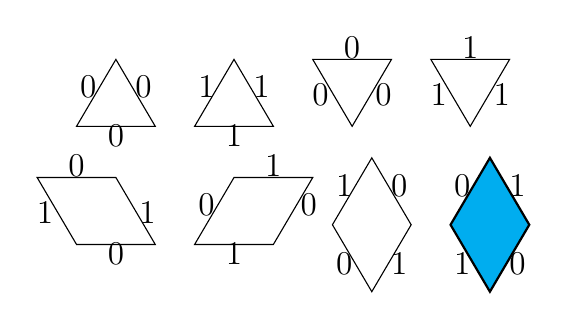
\begin{tikzpicture}[xscale=0.5,yscale=0.5]
      \coordinate (A) at (0,0);
      \coordinate (B) at (2,0);
      \coordinate (C) at (1,1.7);

      \draw (A)--(B)--(C)--cycle;
      \node[font=\large] at ($(A)+(1,-0.25)$) {$0$};
      \node[font=\large] at ($(A)+(0.3,1)$) {$0$};
      \node[font=\large] at ($(A)+(1.7,1)$) {$0$};

      \coordinate(P) at (3,0);
      \draw ($(A)+(P)$)--($(B)+(P)$)--($(C)+(P)$)--cycle;
      \node[font=\large] at ($(P)+(1,-0.25)$) {$1$};
      \node[font=\large] at ($(P)+(0.3,1)$) {$1$};
      \node[font=\large] at ($(P)+(1.7,1)$) {$1$};

      \coordinate (Q) at (6,0);
      \draw ($(A)+(Q)+(0,1.7)$)--($(B)+(Q)+(0,1.7)$)--($(C)+(Q)-(0,1.7)$)--cycle;
      \node[font=\large] at ($(Q)+(0.2,0.8)$) {$0$};
      \node[font=\large] at ($(Q)+(1.8,0.8)$) {$0$};
      \node[font=\large] at ($(Q)+(1,2)$) {$0$};

      \coordinate (R) at (9,0);
      \draw ($(A)+(R)+(0,1.7)$)--($(B)+(R)+(0,1.7)$)--($(C)+(R)-(0,1.7)$)--cycle;
      \node[font=\large] at ($(R)+(0.2,0.8)$) {$1$};
      \node[font=\large] at ($(R)+(1.8,0.8)$) {$1$};
      \node[font=\large] at ($(R)+(1,2)$) {$1$};

      \draw ($(A)-(0,3)$)--($(B)-(0,3)$)--($(C)-(0,3)$)--($(C)-(2,3)$)--cycle; 
      \node[font=\large] at ($(A)+(1,-3.25)$) {$0$};
      \node[font=\large] at ($(A)+(1.8,-2.2)$) {$1$};
      \node[font=\large] at ($(A)+(-0.8,-2.2)$) {$1$};
      \node[font=\large] at ($(A)+(0,-1)$) {$0$};

      \draw ($(A)-(-3,3)$)--($(B)-(-3,3)$)--($(C)-(-5,3)$)--($(C)-(-3,3)$)--cycle;
      \node[font=\large] at ($(P)+(1,-3.25)$) {$1$};
      \node[font=\large] at ($(P)+(2.9,-2)$) {$0$};
      \node[font=\large] at ($(P)+(0.3,-2)$) {$0$};
      \node[font=\large] at ($(P)+(2,-1)$) {$1$}; 

      \draw ($(A)+(6.5,-2.5)$)--($(C)+(6.5,-2.5)$)--($(B)+(6.5,-2.5)$)--($(C)+(6.5,-5.9)$)--cycle;
      \node[font=\large] at ($(Q)+(0.8,-1.5)$) {$1$};
      \node[font=\large] at ($(Q)+(2.2,-1.5)$) {$0$};
      \node[font=\large] at ($(Q)+(2.2,-3.5)$) {$1$};
      \node[font=\large] at ($(Q)+(0.8,-3.5)$) {$0$};

      \fill[cyan] ($(A)+(9.5,-2.5)$)--($(C)+(9.5,-2.5)$)--($(B)+(9.5,-2.5)$)--($(C)+(9.5,-5.9)$)--cycle;
      \draw[thick] ($(A)+(9.5,-2.5)$)--($(C)+(9.5,-2.5)$)--($(B)+(9.5,-2.5)$)--($(C)+(9.5,-5.9)$)--cycle;
      \node[font=\large] at ($(R)+(0.8,-1.5)$) {$0$};
      \node[font=\large] at ($(R)+(2.2,-1.5)$) {$1$};
      \node[font=\large] at ($(R)+(2.2,-3.5)$) {$0$};
      \node[font=\large] at ($(R)+(0.8,-3.5)$) {$1$};
    \end{tikzpicture}
  \end{figure}
  青塗された図形をequivariant pieceという.
  \end{defin}
\end{frame}

\begin{frame}{puzzleによる方法}
  \begin{eg}
    puzzleの例.
    \begin{figure}[htbp]
      \centering
      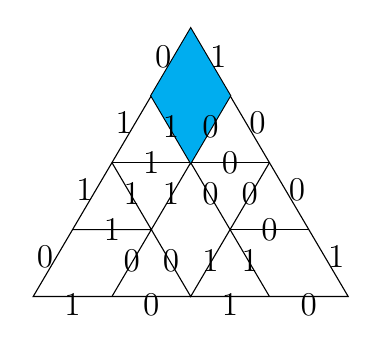
\begin{tikzpicture}[xscale=0.5,yscale=0.5]
        \draw (0,0)--(8,0)--(4,6.8)--cycle;
        \draw (2,0)--(3,1.7)--(1,1.7);
        \draw (3,1.7)--(4,0)--(5,1.7)--(6,0);
        \draw (5,1.7)--(7,1.7);
  
        \draw (2,3.4)--(3,1.7)--(4,3.4)--(5,1.7)--(6,3.4);
        \draw (2,3.4)--(6,3.4);
  
        \draw[thick] (3,5.1)--(4,3.4)--(5,5.1)--(4,6.8)--cycle;
        \fill[cyan] (3,5.1)--(4,3.4)--(5,5.1)--(4,6.8)--cycle;
  
        \node[font=\large] at (1,-0.2) {$1$};
        \node[font=\large] at (3,-0.2) {$0$};
        \node[font=\large] at (5,-0.2) {$1$};
        \node[font=\large] at (7,-0.2) {$0$};
  
        \node[font=\large] at (2,1.7) {$1$};
        \node[font=\large] at (6,1.7) {$0$};
  
        \node[font=\large] at (3,3.4) {$1$};
        \node[font=\large] at (5,3.4) {$0$};
  
  
        \coordinate (A) at (0.3, 1);
        \coordinate (P) at (1,1.7);
        \node[font=\large] at (A) {$0$};
        \node[font=\large] at ($(A)+(P)$) {$1$};
        \node[font=\large] at ($(A)+2*(P)$) {$1$};
        \node[font=\large] at ($(A)+3*(P)$) {$0$};
  
        \coordinate (B) at (7.7, 1);
        \coordinate (Q) at (-1,1.7);
        \node[font=\large] at (B) {$1$};
        \node[font=\large] at ($(B) + (Q)$) {$0$};
        \node[font=\large] at ($(B) + 2*(Q)$) {$0$};
        \node[font=\large] at ($(B) + 3*(Q)$) {$1$};
  
        \node[font=\large] at (2.5,0.9) {$0$};
        \node[font=\large] at (3.5,0.9) {$0$};
        \node[font=\large] at (4.5,0.9) {$1$};
        \node[font=\large] at (5.5,0.9) {$1$};
        
        \node[font=\large] at (2.5,2.6) {$1$};
        \node[font=\large] at (3.5,2.6) {$1$};
        \node[font=\large] at (4.5,2.6) {$0$};
        \node[font=\large] at (5.5,2.6) {$0$};
  
        \node[font=\large] at (3.5,4.3) {$1$};
        \node[font=\large] at (4.5,4.3) {$0$};
      \end{tikzpicture}
    \end{figure}
  \end{eg}
\end{frame}

\begin{frame}{puzzleによる方法}
  \begin{defin}
    puzzle $P$に対して,$P$の周の各辺上の文字を図の方向に読んで得られる文字列をそれぞれ$\lambda,\mu,\nu$とするとき,$\partial P = \Delta^\nu_{\lambda\mu}$と書く.

  \begin{figure}
    \center
    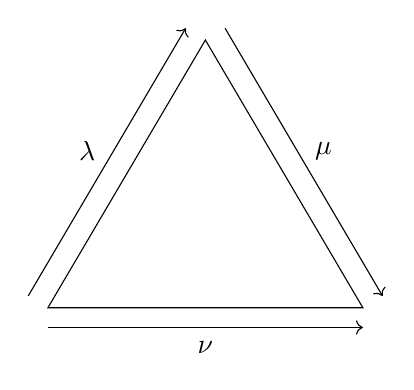
\begin{tikzpicture}[xscale=0.5,yscale=0.5]
      \begin{scope}
        \draw (0,0)--(8,0)--(4,6.8)--cycle;
        \draw[->] (-0.5,0.3) -- ++(4,6.8);
        \node at (2-1,3.4+0.58) {$\lambda$};

        \draw[->] (4+0.5,6.8+0.3) -- ++(4,-6.8);
        \node at (6+1,3.4+0.58) {$\mu$};

        \draw[->] (0,-0.5) -- (8,-0.5);
        \node at (4,-1) {$\nu$};
      \end{scope}
      \begin{scope}
        
      \end{scope}
    \end{tikzpicture}
  \end{figure}
  \end{defin}
\end{frame}

\begin{frame}{puzzleによる方法}
  \begin{eg}
    puzzleの例.
    \begin{figure}[htbp]
      \centering
      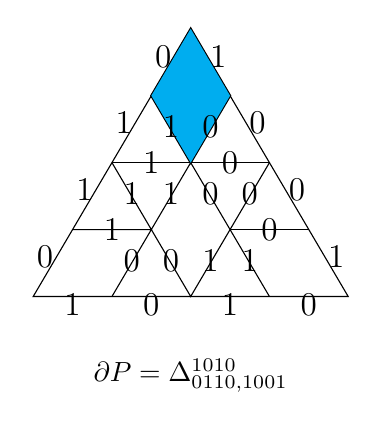
\begin{tikzpicture}[xscale=0.5,yscale=0.5]
        \draw (0,0)--(8,0)--(4,6.8)--cycle;
        \draw (2,0)--(3,1.7)--(1,1.7);
        \draw (3,1.7)--(4,0)--(5,1.7)--(6,0);
        \draw (5,1.7)--(7,1.7);
  
        \draw (2,3.4)--(3,1.7)--(4,3.4)--(5,1.7)--(6,3.4);
        \draw (2,3.4)--(6,3.4);
  
        \draw[thick] (3,5.1)--(4,3.4)--(5,5.1)--(4,6.8)--cycle;
        \fill[cyan] (3,5.1)--(4,3.4)--(5,5.1)--(4,6.8)--cycle;
  
        \node[font=\large] at (1,-0.2) {$1$};
        \node[font=\large] at (3,-0.2) {$0$};
        \node[font=\large] at (5,-0.2) {$1$};
        \node[font=\large] at (7,-0.2) {$0$};
  
        \node[font=\large] at (2,1.7) {$1$};
        \node[font=\large] at (6,1.7) {$0$};
  
        \node[font=\large] at (3,3.4) {$1$};
        \node[font=\large] at (5,3.4) {$0$};
  
  
        \coordinate (A) at (0.3, 1);
        \coordinate (P) at (1,1.7);
        \node[font=\large] at (A) {$0$};
        \node[font=\large] at ($(A)+(P)$) {$1$};
        \node[font=\large] at ($(A)+2*(P)$) {$1$};
        \node[font=\large] at ($(A)+3*(P)$) {$0$};
  
        \coordinate (B) at (7.7, 1);
        \coordinate (Q) at (-1,1.7);
        \node[font=\large] at (B) {$1$};
        \node[font=\large] at ($(B) + (Q)$) {$0$};
        \node[font=\large] at ($(B) + 2*(Q)$) {$0$};
        \node[font=\large] at ($(B) + 3*(Q)$) {$1$};
  
        \node[font=\large] at (2.5,0.9) {$0$};
        \node[font=\large] at (3.5,0.9) {$0$};
        \node[font=\large] at (4.5,0.9) {$1$};
        \node[font=\large] at (5.5,0.9) {$1$};
        
        \node[font=\large] at (2.5,2.6) {$1$};
        \node[font=\large] at (3.5,2.6) {$1$};
        \node[font=\large] at (4.5,2.6) {$0$};
        \node[font=\large] at (5.5,2.6) {$0$};
  
        \node[font=\large] at (3.5,4.3) {$1$};
        \node[font=\large] at (4.5,4.3) {$0$};

        \node at (4,-2) {$\partial P = \Delta^{1010}_{0110,1001}$};
      \end{tikzpicture}
    \end{figure}
  \end{eg}
\end{frame}

\begin{frame}{puzzleによる方法}
  \begin{defin}[puzzleのweight]
    $p$をpuzzle $P$のequivariant pieceとする.図のように$p$から線分を引いたときの$P$の下辺との交点の位置によって$\text{wt}(p)\in\integer[y_1,\cdots,y_n]$を定義する.
  \begin{figure}[htbp]
    \centering
    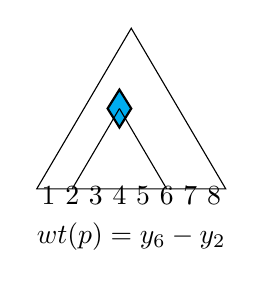
\begin{tikzpicture}[xscale=0.3,yscale=0.3]
      \draw (0,0)--(8,0)--(4,6.8)--cycle;
      \fill[cyan] (3,3.4)--(3.5,2.6)--(4,3.4)--(3.5,4.2)--cycle;
      \draw[thick] (3,3.4)--(3.5,2.6)--(4,3.4)--(3.5,4.2)--cycle;
      
      \draw (3.5,3.4)--(1.5,0);
      \draw (3.5,3.4)--(5.5,0);
  
  
      \node at (0.5,-0.3) {$1$};
      \node at (1.5,-0.3) {$2$};
      \node at (2.5,-0.3) {$3$};
      \node at (3.5,-0.3) {$4$};
      \node at (4.5,-0.3) {$5$};
      \node at (5.5,-0.3) {$6$};
      \node at (6.5,-0.3) {$7$};
      \node at (7.5,-0.3) {$8$};

      \node at (4,-2) {$\text{wt}(p)=y_6-y_2$};
    \end{tikzpicture}
  \end{figure}
  また,$\text{wt}(P) = \prod_{p}\text{wt}(p)$とする.
  \end{defin}
\end{frame}

\begin{frame}{puzzleによる方法}
  \begin{theo}[Knutson-Tao]
    同変Littlewood-Richardson係数$C^\nu_{\lambda\mu}$について
    \[
    C^\nu_{\lambda\mu} = \sum_{\partial P = \Delta^\nu_{\lambda\mu}}\text{wt}(P)
    \]
    が成り立つ.
  \end{theo}
\end{frame}

\section{edge labeled tableauxによる方法}

\begin{frame}{edge labeled tableauxによる方法}
  $\lambda\in\binom{n}{k}$を左から読んで$i_1<\cdots<i_k$番目に$1$が現れるとする.
  \[
  l_a = \#\set{j}{j > i_a, \lambda_j = 0},\quad \text{for }a = 1,\cdots,k
  \]
  によって分割$l=(l_1,\cdots,l_k)$が得られる.この対応によって$\binom{n}{k}$は$((n-k)^k)$に含まれる分割と同一視できる.
  \begin{figure}
    \center
    \begin{tikzpicture}
      \node at (0,0) {$\lambda = 10010$};
      \node at (1.5,0) {$\rightarrow$};

      \begin{scope}[xshift = 2.7cm, yshift = 0.8cm]
        \node at (-0.4,-0.8) {$l=$};
        \draw (0,0) -- ++(2.4,0);
        \draw (0,-0.8) -- ++(2.4,0);
        \draw (0,-1.6) -- ++(0.8,0);
        \draw (0,0) -- ++(0,-1.6);
        \draw (0.8,0) -- ++(0,-1.6); 
        \draw (1.6,0)-- ++(0,-0.8);
        \draw (2.4,0)-- ++(0,-0.8);
      \end{scope}
    \end{tikzpicture}
  \end{figure}
\end{frame}

\begin{frame}{edge labeled tableauxによる方法}
  \begin{defin}[equivariant filling]
    分割$\lambda, \nu$に対して,$\lambda_i\leq\nu_i$がすべての$i$で成り立つとき,$\lambda\leq\nu$とする.このとき$\nu$の箱であって$\lambda$の箱でないもの全体を歪Young図形といい$\nu/\lambda$と書く.

  $\nu/\lambda$の各箱に$1$から$m$までの数字を$1$つ書き入れ,$\lambda$の水平方向の境界から下にある水平方向の各辺に$\{1,\cdots,m\}$の空でもよい部分集合を書き入れたものをequivariant fillingという.
  \end{defin}
\end{frame}

\begin{frame}{edge labeled tableauxによる方法}
  \footnotesize
  \begin{defin}[equivariant standard tableaux]
    形が$\nu/\lambda$のequivariant fillingのうち,次の条件を満たすものをequivariant standard tableauxという.
  \begin{itemize}
    \item $1$から$m$までの各数字が,いずれかの箱のラベルに現れるか,またはいずれかの辺のラベルの要素になっている.また$1$から$m$までの各数字がちょうど1回現れる.
    \item 各箱のラベルについて,左隣の箱のラベルよりも大きい.
    \item 各箱のラベルについて,上辺のラベルが空でないなら,その最大値よりも大きい.空であるならば,すぐ上の箱のラベルより大きい.
    \item 各辺のラベルについて,そのすべての数字がすぐ上の箱に書かれたラベルよりも大きい.
  \end{itemize}
  形が$\nu/\lambda$で$1$から$m$までの数字が書かれたequivariant standard tableauxの全体の集合を$\text{EqSYT}(\nu/\lambda, m)$とする.
  \end{defin}
  \normalsize
\end{frame}

\begin{frame}{edge labeled tableauxによる方法}
  \begin{eg}
    equivariant standard tableauxとそうでないものの例.左図は$\{3,5\}$が$\lambda=(2,2,1)$の境界から下にないためequivariant fillingでない.中央の図は$1$と$2$が$\lambda=(1,1,1)$の境界から下にないためequivariant fillingでない.右図は$(4,4,2)/(3,3,1)$上のequivariant standard tableauxの例である.
  \begin{figure}
    \centering
    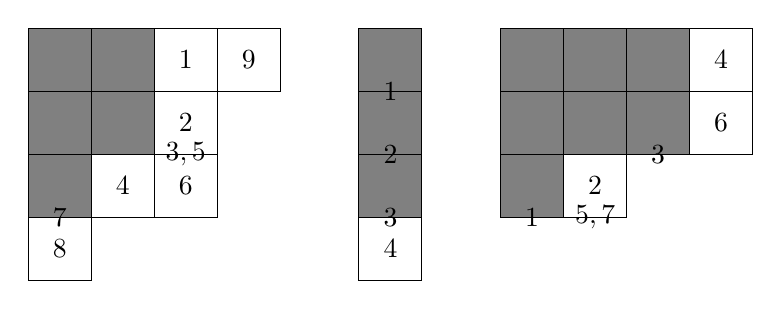
\begin{tikzpicture}
      \begin{scope}
        \fill[gray] (0,0)--(1.6,0)--(1.6,-1.6)--(0.8,-1.6)--(0.8,-2.4)--(0,-2.4)--cycle;
        \draw (0,0)--(0,-3.2)--(0.8,-3.2)--(0.8,-2.4)--(2.4,-2.4)--(2.4,-0.8)--(3.2,-0.8)--(3.2,0)--cycle;
        \draw (0,-0.8)--(2.4,-0.8);
        \draw (0,-1.6)--(2.4,-1.6);
        \draw (0,-2.4)--(0.8,-2.4);
        \draw (0.8,0)--(0.8,-2.4);
        \draw (1.6,0)--(1.6,-2.4);
        \draw (2.4,0)--(2.4,-0.8);
  
        \node at (2,-0.4) {$1$};
        \node at (2.8,-0.4) {$9$};
        \node at (2,-1.2) {$2$};
        \node at (1.2,-2) {$4$};
        \node at (2,-2) {$6$};
        \node at (0.4,-2.8) {$8$};
  
        \node at (0.4,-2.4) {$7$};
        \node at (2,-1.6) {$3,5$};
      \end{scope}
      \begin{scope}[xshift=4.2cm]
        \fill[gray] (0,0) rectangle ++(0.8,-2.4);
        \draw (0,0) rectangle ++(0.8,-3.2);
        \draw (0,-0.8) -- ++(0.8,0);
        \draw (0,-1.6) -- ++(0.8,0);
        \draw (0,-2.4) -- ++(0.8,0);
        
        \node at (0.4,-0.8) {$1$};
        \node at (0.4,-1.6) {$2$};
        \node at (0.4,-2.4) {$3$};
        \node at (0.4,-2.8) {$4$};
      \end{scope}
      \begin{scope}[xshift=6cm]
        \fill[gray] (0,0)--(2.4,0)--(2.4,-1.6)--(0.8,-1.6)--(0.8,-2.4)--(0,-2.4)--cycle;
        \draw (0,0)--(3.2,0)--(3.2,-1.6)--(1.6,-1.6)--(1.6,-2.4)--(0,-2.4)--cycle;
        \draw (0.8,0)-- +(0,-2.4);
        \draw (1.6,0)-- +(0,-1.6);
        \draw (2.4,0)-- +(0,-1.6);
        \draw (0,-0.8)-- +(3.2,0);
        \draw (0,-1.6)-- +(1.6,0);
  
        \node at (2.8,-0.4) {$4$};
        \node at (2.8,-1.2) {$6$};
        \node at (1.2,-2) {$2$};
        \node at (0.4,-2.4) {$1$};
        \node at (1.2,-2.4) {$5,7$};
        \node at (2,-1.6) {$3$};
      \end{scope}
    \end{tikzpicture}
  \end{figure}
  \end{eg}
\end{frame}

\begin{frame}{edge labeled tableauxによる方法}
  \begin{defin}[equivariant jeu de taquin]\label{jeu de taquin}
    \footnotesize
    $T\in\text{EqSYT}(\nu/\lambda,m)$の内隅$x$に対して,$x$が外隅になるまで次の操作を繰り返して得られるtableauxを$x$によるequivariant jeu de taquinといい$\text{EqJdt}_x(T)$と書く.
    \begin{figure}
      \center
      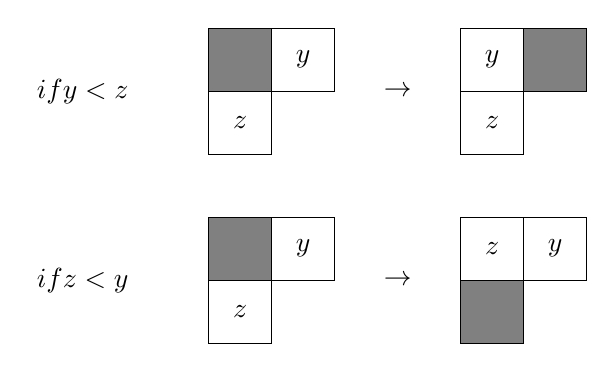
\begin{tikzpicture}
        \begin{scope}
          \node at (-1.6,-0.8) {$\text{if } y < z$};
          \draw[fill=gray] (0,0) rectangle ++(0.8,-0.8);
          \draw (0,0) rectangle ++(0.8,-0.8);
          \draw (0.8,0) rectangle ++(0.8,-0.8);
          \node at (1.2,-0.4) {$y$};
          \draw (0,-0.8) rectangle ++(0.8,-0.8);
          \node at (0.4,-1.2) {$z$};
          \node at (2.4,-0.8) {$\rightarrow $};

          \draw (3.2,0) rectangle ++(0.8,-0.8);
          \draw[fill=gray] (4,0) rectangle ++(0.8,-0.8);
          \draw (4,0) rectangle ++(0.8,-0.8);
          \node at (3.6,-0.4) {$y$};
          \draw (3.2,-0.8) rectangle ++(0.8,-0.8);
          \node at (3.6,-1.2) {$z$};
        \end{scope}
        \begin{scope}[yshift = -2.4cm]
          \node at (-1.6,-0.8) {$\text{if } z < y$};
          \draw[fill=gray] (0,0) rectangle ++(0.8,-0.8);
          \draw (0,0) rectangle ++(0.8,-0.8);
          \draw (0.8,0) rectangle ++(0.8,-0.8);
          \node at (1.2,-0.4) {$y$};
          \draw (0,-0.8) rectangle ++(0.8,-0.8);
          \node at (0.4,-1.2) {$z$};
          \node at (2.4,-0.8) {$\rightarrow $};

          \draw (3.2,0) rectangle ++(0.8,-0.8);
          \draw[fill=gray] (3.2,-0.8) rectangle ++(0.8,-0.8);
          \draw (4,0) rectangle ++(0.8,-0.8);
          \node at (4.4,-0.4) {$y$};
          \draw (3.2,-0.8) rectangle ++(0.8,-0.8);
          \node at (3.6,-0.4) {$z$};
        \end{scope}
      \end{tikzpicture}
    \end{figure}
  \end{defin}
\end{frame}

\begin{frame}{edge labeled tableauxによる方法}
  \begin{block}{定義\ref{jeu de taquin}の続き}
  \begin{figure}
    \center
    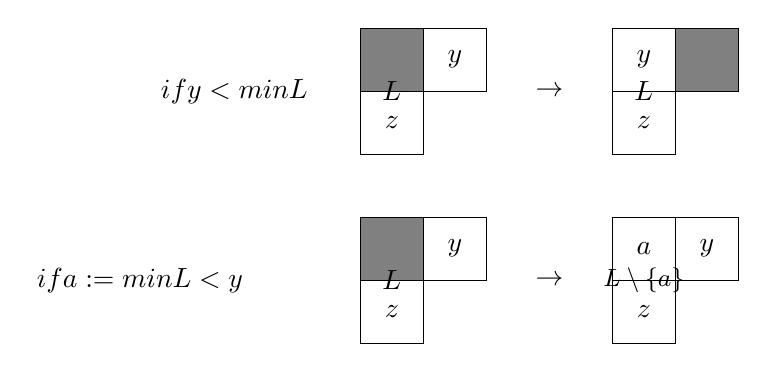
\begin{tikzpicture}
    \begin{scope}
      \node at (-1.6,-0.8) {$\text{if } y < \text{min }L$};
      \draw[fill=gray] (0,0) rectangle ++(0.8,-0.8);
      \node at (0.4,-0.8) {$L$};
      \draw (0,0) rectangle ++(0.8,-0.8);
      \draw (0.8,0) rectangle ++(0.8,-0.8);
      \node at (1.2,-0.4) {$y$};
      \draw (0,-0.8) rectangle ++(0.8,-0.8);
      \node at (0.4,-1.2) {$z$};
      \node at (2.4,-0.8) {$\rightarrow $};

      \draw (3.2,0) rectangle ++(0.8,-0.8);
      \draw[fill=gray] (4,0) rectangle ++(0.8,-0.8);
      \node at (3.6,-0.8) {$L$};
      \draw (4,0) rectangle ++(0.8,-0.8);
      \node at (3.6,-0.4) {$y$};
      \draw (3.2,-0.8) rectangle ++(0.8,-0.8);
      \node at (3.6,-1.2) {$z$};
    \end{scope}
    \begin{scope}[yshift = -2.4cm]
      \node at (-2.8,-0.8) {$\text{if } a:=\text{min }L < y$};
      \draw[fill=gray] (0,0) rectangle ++(0.8,-0.8);
      \node at (0.4,-0.8) {$L$};
      \draw (0,0) rectangle ++(0.8,-0.8);
      \draw (0.8,0) rectangle ++(0.8,-0.8);
      \node at (1.2,-0.4) {$y$};
      \draw (0,-0.8) rectangle ++(0.8,-0.8);
      \node at (0.4,-1.2) {$z$};
      \node at (2.4,-0.8) {$\rightarrow $};

      \draw (3.2,0) rectangle ++(0.8,-0.8);
      \node at (3.6,-0.4) {$a$};
      \node[font=\small] at (3.6,-0.8) {$L\setminus \{a\}$};
      \draw (4,0) rectangle ++(0.8,-0.8);
      \node at (4.4,-0.4) {$y$};
      \draw (3.2,-0.8) rectangle ++(0.8,-0.8);
      \node at (3.6,-1.2) {$z$};
    \end{scope}
  \end{tikzpicture}
  \end{figure}
  \end{block}
\end{frame}

\begin{frame}{edge labeled tableauxによる方法}
  \begin{defin}
    $T\in\text{EqSYT}(\nu/\lambda,m)$に対して,次のような順番でequivariant jeu de taquinを施したtableauxをequivariant rectificationと呼び,$\text{EqRect}(T)$と書く.
    \begin{figure}
      \center
      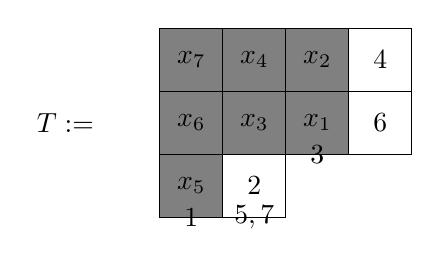
\begin{tikzpicture}
      \fill[gray] (0,0)--(2.4,0)--(2.4,-1.6)--(0.8,-1.6)--(0.8,-2.4)--(0,-2.4)--cycle;
        \draw (0,0)--(3.2,0)--(3.2,-1.6)--(1.6,-1.6)--(1.6,-2.4)--(0,-2.4)--cycle;
        \draw (0.8,0)-- +(0,-2.4);
        \draw (1.6,0)-- +(0,-1.6);
        \draw (2.4,0)-- +(0,-1.6);
        \draw (0,-0.8)-- +(3.2,0);
        \draw (0,-1.6)-- +(1.6,0);
  
        \node at (2.8,-0.4) {$4$};
        \node at (2.8,-1.2) {$6$};
        \node at (1.2,-2) {$2$};
        \node at (0.4,-2.4) {$1$};
        \node at (1.2,-2.4) {$5,7$};
        \node at (2,-1.6) {$3$};

        \node at (2,-1.2) {$x_1$};
        \node at (2,-0.4) {$x_2$};
        \node at (1.2,-1.2) {$x_3$};
        \node at (1.2,-0.4) {$x_4$};
        \node at (0.4,-2) {$x_5$};
        \node at (0.4,-1.2) {$x_6$};
        \node at (0.4,-0.4) {$x_7$};

        \node at (-1.2,-1.2) {$T:=$};
      \end{tikzpicture}
    \end{figure}
    に対して,
    \[
    \text{EqRect}(T) := \text{EqJdt}_{x_7}(\text{EqJdt}_{x_6}(\cdots\text{EqJdt}_{x_1}(T)))
    \]
  \end{defin}
\end{frame}

\begin{frame}{edge labeled tableauxによる方法}
  \begin{eg}
    \begin{figure}[ht]
      \centering
      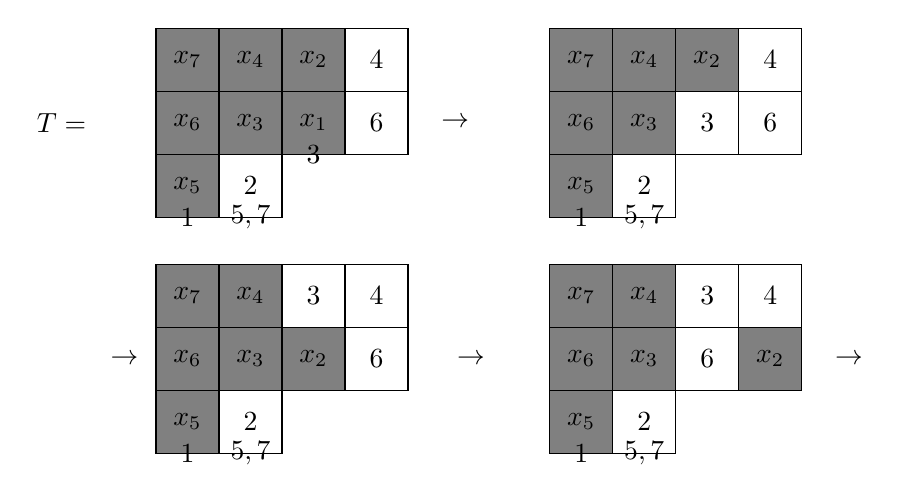
\begin{tikzpicture}
        \begin{scope}
          \fill[gray] (0,0)--(2.4,0)--(2.4,-1.6)--(0.8,-1.6)--(0.8,-2.4)--(0,-2.4)--cycle;
          \draw (0,0)--(3.2,0)--(3.2,-1.6)--(1.6,-1.6)--(1.6,-2.4)--(0,-2.4)--cycle;
          \draw (0.8,0)-- +(0,-2.4);
          \draw (1.6,0)-- +(0,-1.6);
          \draw (2.4,0)-- +(0,-1.6);
          \draw (0,-0.8)-- +(3.2,0);
          \draw (0,-1.6)-- +(1.6,0);
    
          \node at (2.8,-0.4) {$4$};
          \node at (2.8,-1.2) {$6$};
          \node at (1.2,-2) {$2$};
          \node at (0.4,-2.4) {$1$};
          \node at (1.2,-2.4) {$5,7$};
          \node at (2,-1.6) {$3$};
  
          \node at (2,-1.2) {$x_1$};
          \node at (2,-0.4) {$x_2$};
          \node at (1.2,-1.2) {$x_3$};
          \node at (1.2,-0.4) {$x_4$};
          \node at (0.4,-2) {$x_5$};
          \node at (0.4,-1.2) {$x_6$};
          \node at (0.4,-0.4) {$x_7$};
  
          \node at (-1.2,-1.2) {$T=$};
          \node at (3.8,-1.2) {$\rightarrow $};
        \end{scope}
        \begin{scope}[xshift=5cm]
          \fill[gray] (0,0)--(2.4,0)--(2.4,-0.8)--(1.6,-0.8)--(1.6,-1.6)--(0.8,-1.6)--(0.8,-2.4)--(0,-2.4)--cycle;
          \draw (0,0)--(3.2,0)--(3.2,-1.6)--(1.6,-1.6)--(1.6,-2.4)--(0,-2.4)--cycle;
          \draw (0.8,0)-- +(0,-2.4);
          \draw (1.6,0)-- +(0,-1.6);
          \draw (2.4,0)-- +(0,-1.6);
          \draw (0,-0.8)-- +(3.2,0);
          \draw (0,-1.6)-- +(1.6,0);
    
          \node at (2.8,-0.4) {$4$};
          \node at (2.8,-1.2) {$6$};
          \node at (1.2,-2) {$2$};
          \node at (0.4,-2.4) {$1$};
          \node at (1.2,-2.4) {$5,7$};
  
          \node at (2,-1.2) {$3$};
          \node at (2,-0.4) {$x_2$};
          \node at (1.2,-1.2) {$x_3$};
          \node at (1.2,-0.4) {$x_4$};
          \node at (0.4,-2) {$x_5$};
          \node at (0.4,-1.2) {$x_6$};
          \node at (0.4,-0.4) {$x_7$};
  
          
        \end{scope}
        \begin{scope}[yshift = -3cm]
          \node at (-0.4,-1.2) {$\rightarrow $};
          \fill[gray] (0,0)--(1.6,0)--(1.6,-1.6)--(0.8,-1.6)--(0.8,-2.4)--(0,-2.4)--cycle;
          \fill[gray] (1.6,-0.8) rectangle (2.4,-1.6);
          \draw (0,0)--(3.2,0)--(3.2,-1.6)--(1.6,-1.6)--(1.6,-2.4)--(0,-2.4)--cycle;
          \draw (0.8,0)-- +(0,-2.4);
          \draw (1.6,0)-- +(0,-1.6);
          \draw (2.4,0)-- +(0,-1.6);
          \draw (0,-0.8)-- +(3.2,0);
          \draw (0,-1.6)-- +(1.6,0);
    
          \node at (2.8,-0.4) {$4$};
          \node at (2.8,-1.2) {$6$};
          \node at (1.2,-2) {$2$};
          \node at (0.4,-2.4) {$1$};
          \node at (1.2,-2.4) {$5,7$};
  
          \node at (2,-1.2) {$x_2$};
          \node at (2,-0.4) {$3$};
          \node at (1.2,-1.2) {$x_3$};
          \node at (1.2,-0.4) {$x_4$};
          \node at (0.4,-2) {$x_5$};
          \node at (0.4,-1.2) {$x_6$};
          \node at (0.4,-0.4) {$x_7$};

          \node at (4,-1.2) {$\rightarrow$};
        \end{scope}

        \begin{scope}[xshift=5cm,yshift=-3cm]
          \fill[gray] (0,0)--(1.6,0)--(1.6,-1.6)--(0.8,-1.6)--(0.8,-2.4)--(0,-2.4)--cycle;
          \fill[gray] (2.4,-0.8) rectangle (3.2,-1.6);
          \draw (0,0)--(3.2,0)--(3.2,-1.6)--(1.6,-1.6)--(1.6,-2.4)--(0,-2.4)--cycle;
          \draw (0.8,0)-- +(0,-2.4);
          \draw (1.6,0)-- +(0,-1.6);
          \draw (2.4,0)-- +(0,-1.6);
          \draw (0,-0.8)-- +(3.2,0);
          \draw (0,-1.6)-- +(1.6,0);
    
          \node at (2.8,-0.4) {$4$};
          \node at (2.8,-1.2) {$x_2$};
          \node at (1.2,-2) {$2$};
          \node at (0.4,-2.4) {$1$};
          \node at (1.2,-2.4) {$5,7$};
  
          \node at (2,-1.2) {$6$};
          \node at (2,-0.4) {$3$};
          \node at (1.2,-1.2) {$x_3$};
          \node at (1.2,-0.4) {$x_4$};
          \node at (0.4,-2) {$x_5$};
          \node at (0.4,-1.2) {$x_6$};
          \node at (0.4,-0.4) {$x_7$};

          \node at (3.8,-1.2) {$\rightarrow $};
        \end{scope}
      \end{tikzpicture}
    \end{figure}
  \end{eg}
\end{frame}

\begin{frame}{edge labeled tableauxによる方法}
  $T\in\text{EqSYT}(\nu/\lambda)$に対して,次のようにweightを定義する.
  \begin{defin}[Manhattan距離]
    $\Lambda = ((n-k)^k)$の各箱$x$に対して,$d(x)$を図のように定める.すなわち$d(x)$は$\Lambda$の右上の隅の箱と$x$とのManhattan距離(に$1$を加えたもの)に等しい.
    \[
  \begin{ytableau}
    4 & 3 & 2 & 1\\
    5 & 4 & 3 & 2\\
    6 & 5 & 4 & 3
  \end{ytableau}
  \]
  \end{defin}
\end{frame}

\begin{frame}{edge labeled tableauxによる方法}
  \begin{defin}[tableauxのweight]
    \small
    $l\in\integer$が$T$の辺のラベルに現れるとする.$l$を含む列に存在する$\lambda$の箱をすべてjeu de taquinする課程で$l$が通る箱を下から順に$z_{1},\cdots,z_{s}$とし,$z_{s}$と同じ行にある箱のうち最も右にある箱を$w$とする.$i = d(z_1) + 1$, $j = d(w)$として
    \[
    \text{factor}(l) = y_i - y_j
    \]
    とする.$l$が箱のラベルに入らないときは$\text{factor}(l) = 0$とする.
    $T$のweightを
    \[
    \text{wt}(T) = \prod_{l:\text{ edge label of }T} \text{factor}(l)
    \]
    と定義する.
  \end{defin}
  \normalsize
\end{frame}

\begin{frame}
  \begin{theo}[Knutson-Tao]
    同変Littlewood-Richardson係数$C^\nu_{\lambda\mu}$について
    \[
    C^\nu_{\lambda\mu} = \sum_{\substack{
      T\in\text{EqSYT}(\nu/\lambda,|\mu|)\\
      \text{EqRect}(T) = T_\mu\\
      \text{wt}(T)\neq 0
    }}\text{wt}(T)
    \]
    が成り立つ.
    ここで$T_\mu$は形が$\mu$のstandard tableauxで,$1$行目から順に左から$1,2,\cdots,|\mu|$を書き入れたものである.
  \end{theo}
\end{frame}


\section{等価性}

\begin{frame}{等価性}
  紹介した2つの数え上げは本質的に同じであることが示せる.すなわち,
  $\mathcal{P}^\nu_{\lambda\mu}=\set{P:\text{ puzzle}}{\partial P = \Delta^\nu_{\lambda\mu}}$,$\mathcal{T}^\nu_{\lambda\mu} = \set{T\in\text{EqSYT}(\nu/\lambda,|\mu|)}{\text{EqRect}(T)=T_\mu,\text{wt}(T)\neq 0}$としたとき,次が成り立つ.
  \begin{theo}\label{main theorem}
    全単射$\varphi:\mathcal{P}^\nu_{\lambda\mu}\rightarrow \mathcal{T}^\nu_{\lambda\mu}$であって$\text{wt}(\varphi(P))=\text{wt}(P)$を満たすものが存在する.
  \end{theo}
\end{frame}

\begin{frame}
  定理\ref{main theorem}の$\varphi$は次のように構成される.
\end{frame}


\end{document}